\chapter{Potential Leakage Sources}

In this chapter, we discuss the potential leakage sources in the environment we have set up in \Cref{Chp: Experiment Setup}. 

\section{Subject} \label{Sec: Subjects}

Without loss of generality, in this report, we are interested in leakages with respect to the following subjects:

\begin{itemize}
	\item Content and size of encrypted data
	\item Cryptographic key materials
	\item Network topology
\end{itemize}

In this chapter we give a theoretical analysis of the exploitable side channel information in the WSN traffic. The inspection of protocol and implementation flaws are included in later chapters.

Notice that Traffic Analysis is highly application specific. In this report, our discussions are based the simple applications described in \Cref{Sec: Applications}. 

\section{Observables} \label{Sec: Observables}

As we have explained in \Cref{Chp: Experiment Setup}, we assumed the adversary has full access to all traffic being transmitted in the WSN. 

\begin{figure*}[h!]
	\center
	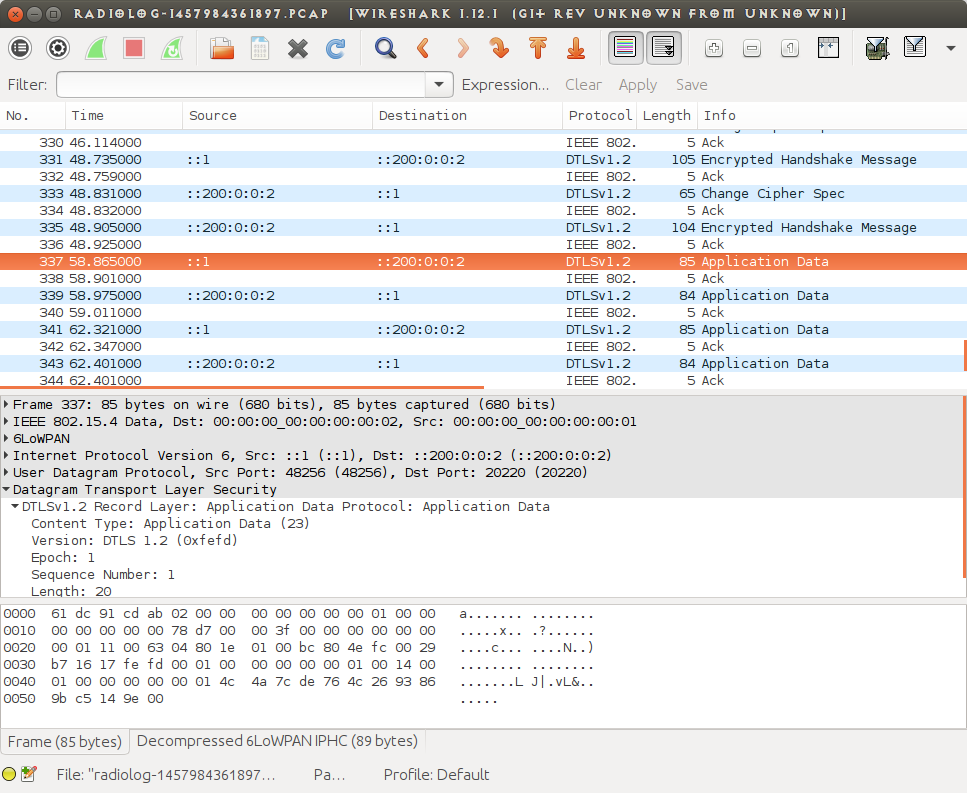
\includegraphics[width=0.9\textwidth]{fig/udpexample.png}
	\caption{An Example of Captured Traffic}
	\label{Fig: An Example of Captured Traffic}
\end{figure*}

\Cref{Fig: An Example of Captured Traffic} shows the packets captured in a Cooja experiment, analysed by Wireshark\cite{Wireshark}. In this research, we assume the value of ciphertext is independent to the plaintext and key. The following side channel information are available in the captured traffic shown in \Cref{Fig: An Example of Captured Traffic}:

\begin{description}[style=nextline]
	\item[Unencrypted headers]
	
	\item[Timing]
	\item[Length]
\end{description}

The timing and length information are always available in the captured traffic. The unencrypted headers depend on the security measure adopted, which we explain in later sections.

Practically, the Receive Signal Strength Indicator, RSSI, should also be considered visible to the adversary. RSSI represents the RF signal strength. By measuring the RSSI of frames sent from a specific source MAC address,  it is possible to reveal the geographical information of a specific Sensor Node. However we do not consider RSSI in this report as its physical character is beyond the scope of this project. Instead, we assume the adversary has prior knowledge of all geographic information of Sensor Nodes in the WSN.

%\subsubsection{noncoresec} \label{Subsubsec: noncoresec header}
%
%As explained in \Cref{Subsec: 802.15.4 Security Implementation in Contiki}, noncoresec is the 802.15.4 Security implementation on Contiki. When noncoresec is enabled, all captured frames are in the form we explained in \Cref{Subsec: 802.15.4 MAC} and \Cref{Subsec: 802154 Sec}. The 802.15.4 MAC Header is the only unencrypted part of a packet.
%
%We stated in \Cref{Subsec: noncoresec in experiment} that we always use the highest Security Level of 802.15.4 Security; therefore:
%\begin{itemize}
%	\item MAC Payload is always authenticated and encrypted in AES-128 with CCM* mode.
%	\item Security Level is constantly 0x7.
%	\item Key Strategy is constantly 0x0 as noncoresec does not implement any key management.
%\end{itemize}
%
%As a result of MAC Payload being authenticated and encrypted, 
%\begin{itemize}
%	\item The adversary cannot join the 6LoWPAN network as we have explained in \Cref{Subsec: noncoresec in experiment}.
%	\item The adversary cannot directly distinguish an IPv6 packet and an ICMPv6 packet by the contents in MAC Payload as it is encrypted. 
%\end{itemize}
%
%%In our experiments, the application data is effectively sent in IPv6 packets. ICMPv6 packets on the other hand are mostly RPL messages.
%
%\subsubsection{DTLS} \label{Subsubsec: DTLS header}
%
%As explained in \Cref{Chp: Building Blocks}, when DTLS is used, the explicit observables are: 
%
%\begin{itemize}
%	\item 802.15.4 MAC Header as explained in \Cref{Subsec: 802.15.4 MAC}.
%	
%	\item Compressed IPv6 Header as explained in \Cref{Subsec: 6LoWPAN Adaptation Sub Layer}, \Cref{Subsec: IPv6 Data Packets} and \Cref{Subsec: ICMPv6}.
%	
%	\item UDP Header as explained in \Cref{Subsec: UDP}.
%	
%	\item DTLS Header as explained in \Cref{Subsec: DTLS}.
%\end{itemize}
%
%Since DTLS is built on Application Layer, therefore it does not impose any setting to the lower layer headers. 

\section{Packet Traces} \label{Sec: Packet Traces}

In this section, we discuss some features of packet traces in WSN applications.

%Before discussing the ``traces'' in WSN applications, as a comparison, we review the different definition of ``traces'' in the literatures we reviewed in \Cref{Chp: Literature Review}:
%
%\begin{itemize}
%	\item In literatures about Traffic Analysis Attacks against web applications\cite{WebSideChannel}\cite{PinpointWeb}\cite{SearchAttack}, a ``trace'' refers to the continuous\footnote{We would argue that the term ``continuous'' is ambiguous; nevertheless it is the best definition we can thought of.} packets triggered by an user input.
%	\item In Website Fingerprinting literatures\cite{WebsiteFingerprint} \cite{HClassifier} \cite{PClassifier} \cite{Peekaboo}, a ``trace'' refers to the continuous packets that triggered by a browser requesting a website.
%	\item Other attacks use more specific application dependent definitions of a ``trace''. \cite{VoIPLanguage} and \cite{VoIPPhrases} defined a ``trace'' to be the continuous packets during a VoIP conversation. \cite{Video} defines it to be the continuous packets during a video conversation. \cite{AppleMessage} does not even use the term ``trace'' at all\footnote{Actually it did used once as a verb equivalent to ``track''.} as it only analyses a single packet.
%\end{itemize}
%
%Practically, the ``trace'' of an Internet application can be defined by filtering packets belong to the same TCP connection,or UDP packets with the same entities\footnote{An entity is the combination of an IP address and a port}. However, we cannot apply the same method on many WSN applications due to the change of protocol suite and application nature. For example, TCP is not used as explained in \Cref{Chp: Building Blocks} and communication are mostly done with ephemeral ports. Further more, the WSN applications perform Machine To Machine, M2M, communication which has much less external intervention, makes it harder to group packets into ``traces''.

WSN application designs tend to be simple and stateless by its nature of constrained resources and underlining protocol suite. In another word, data transmission is minimised for efficiency and data exchanging need be idempotent to maintain robustness. From this aspect, we argue that the simple applications we developed in \Cref{Sec: Applications} have captured these most significant characteristics of WSN applications.

In this report, we define a generic model for the data exchanging process in the WSN applications.

\begin{definition} \label{Def: Session}
A Session is defined as a series of events where a Sensor Node reports application data to a Manager. A Session includes an optional Request sent from Manager to Sensor Node, and a Response containing the requested data sent from Sensor Node to Manager.
\end{definition}

\begin{definition} \label{Def: Trace}
A trace is defined as all captured packets within one Session.
\end{definition}

Although not necessary under \Cref{Def: Session}, in most of our applications, there are typically one or two packets in a trace. The first one corresponds to Request and the second corresponds to Response. In some applications such as broadcast keyllsec in \Cref{Sec: Applications} or a CoAP application using OBSERVE option in \Cref{Subsec: CoAP}, there might be only one Response packet in a trace without a Request. In real world applications there might even be a Request without a Response, e.g. a command to control a light bulb. However, in this report, we define there is at least one packet corresponds to Response. We further assume the adversary is aware of the application running on the Sensor Nodes. Consequently, the adversary in our setting is able to distinguish a Request and a Response, but has no knowledge of the application data being transmitted within them.

We also assume the adversary is capable to distinguish Sessions. Practically, the time interval of packets within the same Session are usually significantly less then the interval between Sessions. \Cref{Fig: Example Traces of keyllsec} shows an example of traces in a unicast keyllsec application instance. Marked are packets for two continuous Sessions, where No.977 and No.990 is the first Session and No.998 and No.1011 are the second. We can see that the time interval within a Session is about 150ms which is significantly less than the 15s interval between Sessions.

\begin{figure*}[h!]
	\center
	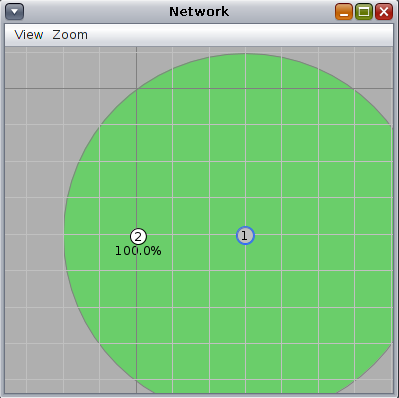
\includegraphics[width=0.5\textwidth]{fig/unicast_keyllsec.png}
	\\
	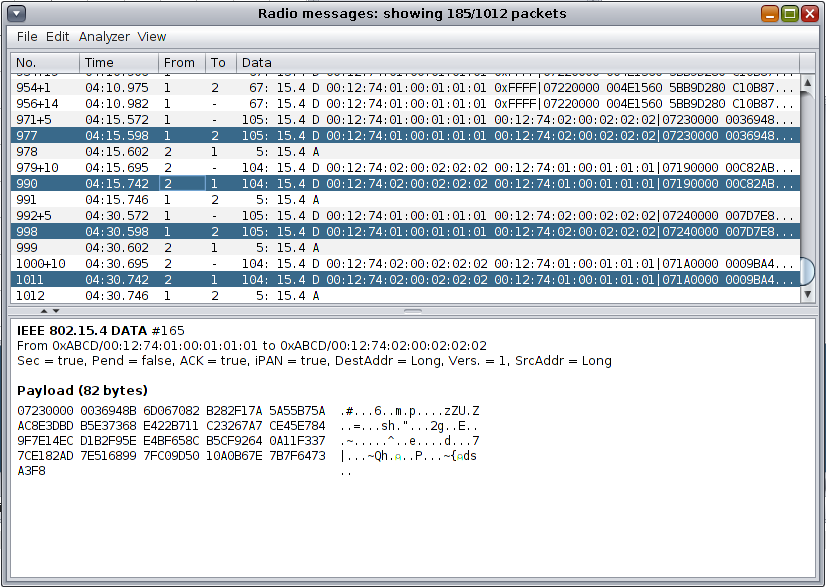
\includegraphics[width=0.9\textwidth]{fig/trace_keyllsec.png}
	\caption{
		Example Traces of keyllsec, \textcircled{1} is the sender and \textcircled{2} the receiver.
	}
	\label{Fig: Example Traces of keyllsec}
\end{figure*}

In this project, we consider only information leakage within one Session. It is arguably that there is potential leakage when jointly analyse traces from different Sessions, e.g. the frequency of Requests can ``leak'' itself. However, we omit such leakage for generality as exploiting them requires further assumptions to the higher level application. Each Session in this report is also considered to be independent based on that fact that each execution of our code is independent to its last execution.

%Further more, in our applications the content of Request is a constant 3 bytes ASCII string ``GET''. We assume this known by the adversary. We make this assumption to focus on the leakage of the Application Data in Responses. 

\section{Theoretical Analysis} \label{Sec: Theoretical Analysis}

In this section we provide a theoretical analysis over all observables we explained in \Cref{Sec: Observables}. It is done in two approaches:

\begin{enumerate}
	\item Cross reference the intersection of the observables we explained in \Cref{Sec: Observables} with the known exploitable side channel information we introduced in \Cref{Sec: Traffic Analysis Attacks}
	\item Semantically analyse the observables. 
\end{enumerate}

%We discuss only the leakage over the attributes we specified in \Cref{Sec: A Review of Review}.

For some of the observables, we claim:

\begin{theorem} \label{Te: IR}
Under the leakage definitions of Mutual Information and g-leakage in \Cref{Subsec: Information Theory}, if an observable $Y$ is independent to a secret $X$, then there is $0$ leakage of $X$ over $Y$.
\end{theorem}

\Cref{Te: IR} intuitively holds. A formal proof is given in \Cref{Prf: IR}.

\begin{corollary} \label{Cor: Constant Leakage}
	An observable $Y$ with a constant value has no leakage under the leakage definitions of  Mutual Information and g-leakage in \Cref{Subsec: Information Theory}.
\end{corollary}

\begin{proof}
	This directly followed by the fact that a constant $y \in Y$ with $P(y) = 1$ is independent to the secret $X$.
\end{proof}

\subsection{Cross Reference of Observables with Known Attacks} \label{Subsec: Cross Reference}

Despite the differences in the nature applications, we discuss the applicability of the packet features those have been exploited in Traffic Analysis Attacks, as we have summarised in \Cref{Tbl: Classifiers in Traffic Analysis Literatures}.

As a result, we only found four features applicable in our settings:
\begin{itemize}
	\item Packet size
	\item Total bytes
	\item Total Time (only for two packets Session)
	\item Total Per-direction Bandwidth
\end{itemize}

All other features have reduced to a constant or not applicable in our settings. The detailed analysis is described in \Cref{Detail Cross Reference}.

\subsection{Semantic Analysis}

In this section, we analysis the observables based on their semantics. The definitions of headers are explained in \Cref{Chp: Building Blocks}.

\subsubsection{Packet Size}

%Linear relationship of length
We noticed that both noncoresec and DTLS use AES-128 with CCM mode to encrypt their payload. As a nature of a stream cipher, the data is not padded. This effectively indicates that the length of plaintext and ciphertext are expected to have a linear relationship with slope ratio $1$:

\begin{equation} \label{Eq: Linear Length}
	l_{C} = l_{P} + b
\end{equation}

where $l_{C}$ and $l_{P}$ are the length in bytes for packets with and without encryption, and $b$ is a predictable constant induced by security measures such as MIC and additional headers. Practically when the security measure increases the packet size to a value exceeding MTU, the packet will be immediately dropped. We assume plaintext is always in a reasonable length that does not result into a ciphertext exceeding MTU; otherwise the packets cannot be sent and the WSN loses its functionality.

From a leakage perspective, it is obvious that all bits of $l_P$ is leaked by $l_C$. A formal quantification of this leakage is given in \Cref{Linear Leakage}.

\subsubsection{Timing}

Timing information is another important side channel information in WSN traffic. Comparing to Internet applications, we consider timing information as a even more crucial leakage source in WSN for two reasons:

\begin{enumerate}
	\item The timing can be measured more accurate in WSN. Packet traces on Internet are usually measured at one side of the communication therefore the noise induced by RTT must be considered, whereas in the WSN scenario the timing can be measured at each side, removing the noise of RTT.
	\item The low performance of the WSN devices potentially increases the resolution of timing information, i.e. the differences of execution time will be more distinguishable on these devices.
\end{enumerate}

However, timing information would be hard to exploit without precise knowledge of the code running on the target Sensor Node. Several protocol may also affect the measuring of timing, .e.g. ContikiMAC turns off the radio for most of the time and therefore preprocessing the traces is required to measure the timing information for packets.

\subsubsection{Headers with noncoresec}

When noncoresec is enabled, the 802.15.4 MAC Header is the only visible part in all Data Frames. In conclusion, we have not identify any obvious leakage source in the MAC Header that links to our application data. 

%Address
However, in the experiments we realised that the Address Information combined with some other packet features can be used distinguish the RPL messages from the application packets.

Details of the semantic analysis of 802.15.4 MAC Header is given in \Cref{Detail noncoresec Header}. 

\subsubsection{Headers with DTLS}

DTLS is built over UDP; therefore visible headers are 802.15.4 MAC header, compressed IPv6 Header, UDP header and DTLS header. In conclusion, we neither found any obvious value that links to our application data.

Two thing should be noticed when DTLS is the security measure:
\begin{enumerate}
	\item Currently DTLS does not support any form of multicast; therefore when DTLS is used, the destination address can only be a unicast address. 

	\item DTLS protects only application data, the ICMP messages, including RPL messages, are transmitted in plaintext.
\end{enumerate}

Even though DTLS can only be used on unicast communications in our applications, proposals such as \cite{DtlsMulticast1} \cite{DtlsMulticast2} has been made to adapt DTLS to multicast; therefore it is reasonable to expect that the family\footnote{Unicast and multicast. Broadcast is treated as an instance of multicast in IPv6.} of destination address can be a hint to the contents of data encrypted by DTLS in the future. However, we do not discuss this topic further as multicast on DTLS is not implemented yet.

Also to be noticed is that the size of compressed IPv6 Header is variable. Since most of the options are not available in our platform, the variance is most likely to be caused by the use of different modes of addresses. However, all our experiments are set up with the same mode addresses and therefore the compressed IPv6 Header effectively resulted into a constant size.

Details of semantic analysis of the visible headers within DTLS is given in \Cref{Detail DTLS Header}. 

\subsection{Conclusion}

In conclusion, the packet size and timing information are still likely to be the most exploitable side channel information in WSN, just as those attacks on Internet. However, the address information is a potential leakage source in WSN applications.

\section{Leakage of Network Topology} \label{Sec: Leakage of Network Topology}

As explained in \Cref{Sec: Observables}, the geographical information of Sensor Nodes can be detected from the RSSI. Based on this information, topology of the 6LoWPAN network can be deduced in the following ways:

\begin{enumerate}
	%With noncoresec
	\item Within noncoresec, the RPL messages are encrypted. However, the source and destination address information is still visible to the adversary; therefore the connectivity between Sensor Nodes can be estimated based on these information.
	%With DTLS
	\item Within DTLS, the RPL messages are not encrypted. The adversary can reconstruct the network topology from the captured RPL messages.
\end{enumerate}

\section{Summary}

In this chapter, we started by specifying the subjects of information leakage, namely the content and size of application data, cryptographic key materials and network topology in \Cref{Sec: Subjects}. Then we demonstrated an example of captured data and pointed out the available information to an adversary in \Cref{Sec: Observables}. From there, we provided a definition of Sessions in WSN applications and the discussed the form of packet traces in our applications in \Cref{Sec: Packet Traces}.

In \Cref{Sec: Theoretical Analysis}, we gave a theoretical analysis of the observables in WSN traffic. Packet size and timing information turned out to be the likely most exploitable feature even in WSN, while unencrypted address information can also be a hint to the contents in the encrypted data.

With respect to network topology, the unencrypted 802.15.4 MAC Header within noncoresec can be used to estimate the connectivity between Sensor Nodes. DTLS does not protect the RPL messages thus an adversary can reconstruct the network topology from the RPL messages transmitted in plaintext.